\documentclass{llncs}
\usepackage{amssymb}
\usepackage[utf8]{inputenc}
\usepackage{url}
\usepackage{graphicx}
\usepackage{caption}
\usepackage{subcaption}
\usepackage{epstopdf}
\usepackage{subfig}
\usepackage{float}
\usepackage{amsmath}
\usepackage{wrapfig}
\usepackage{fancyhdr} %Usado para configurar encabezado y pie de página
\usepackage{enumitem}
%\usepackage[tight,scriptsize,centerlast]{subfigure}
\usepackage{subfloat} 
%\usepackage{subfigure}



\pagestyle{empty}
\pagestyle{fancy}
%\rfoot{\thepage}

\begin{document}

\title{Pumas@Home 2018 Team Description Paper
\thanks{Acknowledgment: This work was supported by PAPIIT-DGAPA UNAM under Grant IG100915}}
\author{
	Jesus Savage 
	\and Reynaldo Martell 
	\and Hugo Estrada 
	\and Marco Negrete 
	\and Julio Cruz 
	\and Jesus Cruz
	\and Jose Cruz
	\and Edgar Vazquez
	\and Jaime Marquez
	\and Edgar Silva
	\and Manuel Pano 
	\and Luis Alvarez
	\and Mauricio Matamoros
}
\institute{Bio-Robotics Laboratory, School of Engineering \\ National Autonomous University of Mexico \\
\texttt{http://biorobotics.fi-p.unam.mx}}
\maketitle


%%%%%%%%%%%%%
%%%  ABSTRACT  %%%
%%%%%%%%%%%%%
\begin{abstract}

This paper describes the service robot Justina of team Pumas that has participated in the @Home category of the RoboCup and RoCKIn, both of them international competitions; as well as our latest applied research. These competitions had influenced our architecture in the development of better systems for our service robots by developing algorithms to natural language understanding, facial detection through multiple images using RGB cameras and the sound source localization (SSL). 
In our robotics architecture, the VIrtual and Real roBOt sysTem (VIRBOT), the operation of service robots is divided into several subsystems, each of them has a specific functionality  that contributes to the final operation of the robot.
By combining symbolic AI with digital signal processing techniques a good performance of a service robot is obtained.

\end{abstract}

%%%%%%%%%%%%%%%
%%% INTRODUCTION %%%
%%%%%%%%%%%%%%%

\section{Introduction}

Service robots are hardware and software systems that assist humans to perform daily tasks in complex environments, to achieve this: they have to be able to understand spoken or gesture commands from humans; to be able to avoid static and dynamic obstacles while navigating in known and unknown environments; to be able to recognize and to manipulate objects and performing several other tasks that a person might request. 

Our team has been participated in the category @Home continuously since the start of this competition at the RoboCup in Bremen in 2006. Our team obtained the third place in Atlanta in 2007, and has reached the finals in 2014 and 2015, last year, in the RoboCup 2017, the team obtained the fourth place and got the award for the best in Speech Recognition and Natural Language Understanding.

The paper is organized as follows:
section \ref{sec:background} enumerates the hardware and software components of our robot
Justina; section \ref{sec:CurrentResearch}  presents overview of the latest research developments in our
laboratory; and finally, in section \ref{sec:conclusions}, the conclusions and future work are given.


\section{Justina's Robotics Architecture}\label{sec:background}
\subsection{Hardware Configuration}

Our service robot Justina, see figure \ref{fig:justina}, has the following hardware configuration:\\

\begin{wrapfigure}{r}{0.5\textwidth}
	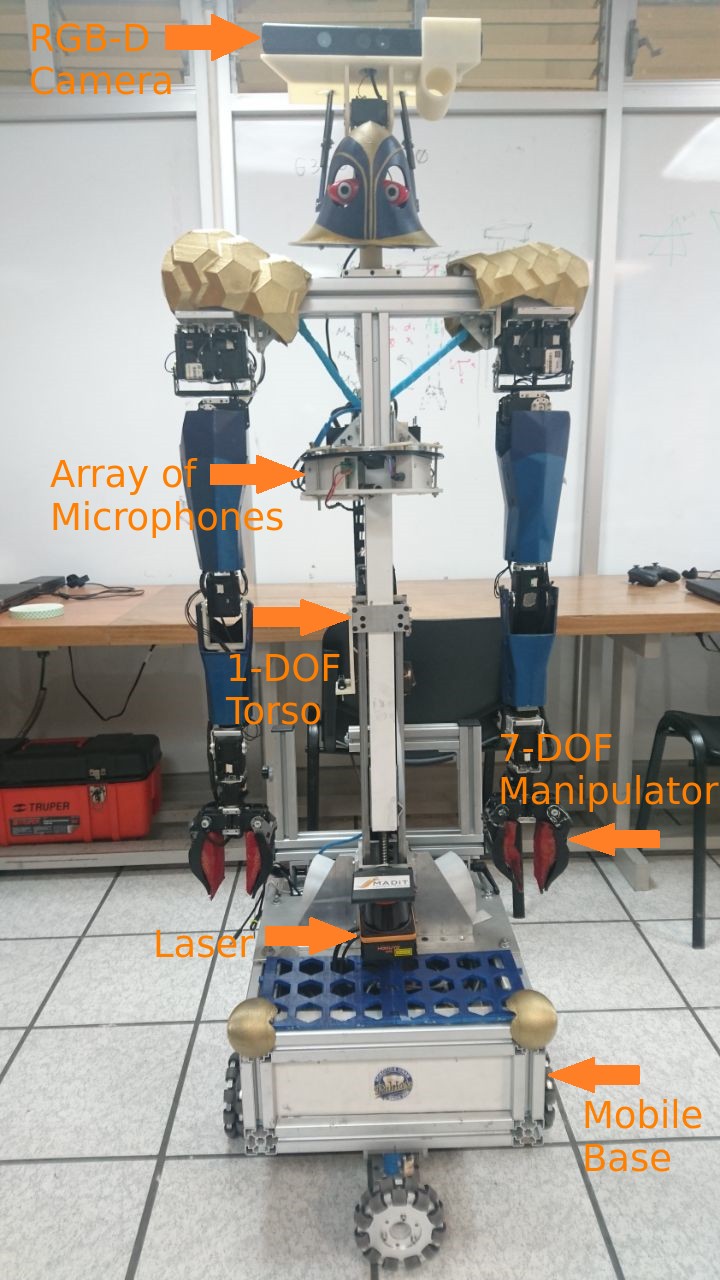
\includegraphics[angle=0, height=11cm, width=6cm]{Figures/justina_scheme.png}
  \caption{Robot Justina}
  \label{fig:justina}
\end{wrapfigure}



ACTUATORS:

\begin{itemize}
	\item \textbf{Mobile base:} Omnidirectional through differential pair configuration and omnidirectional wheels. 
	\item \textbf{Manipulators:} 2 x 7-DOF anthropomorphic arms with 10 Dynamixel servomotors each.
	\item \textbf{Head:} 2-DOF (Pan and tilt) built with Dynamixel servomotors.
	\item \textbf{Torso:} 1-DOF (Elevation) through a worm screw and a configuration of gears. 
	\item \textbf{Speakers:} Two speakers to generate synthetic speech.
\end{itemize}

SENSORS:

\begin{itemize}
	\item \textbf{RGB-D Camera:} Microsoft's Kinect sensor 
	\item \textbf{RGB Camera:} Logitech Pro C920 Full HD.
	\item \textbf{Microphone:} Rode NTG2 directional microphone.
	\item \textbf{Array of Microphones:} An array of four microphones to detect sound sources.
	\item \textbf{Laser:} Hokuyo rangefinder URG-04LX-UG0.
\end{itemize}

\subsection{Software Configuration}
Our software configuration is based on the VIRBOT architecture \cite{virbot}, 
which provides a platform for the design and development of software for general purpose service robots, see figure \ref{fig:virbot}. 
The VIRBOT architecture is implemented in our robots through several modules that perform well defined tasks \cite{muller}, with a 
high level of interaction between them. The principal framework used for interaction is ROS, where a module is represented by one or 
several ROS's nodes. Also, for modules using the Microsoft operating system, we use our own middleware called Blackboard to
link them with ROS nodes running on Linux.
In the following sections are explained each of the layers of the VIRBOT system.


\begin{figure}[h]
	\centering
	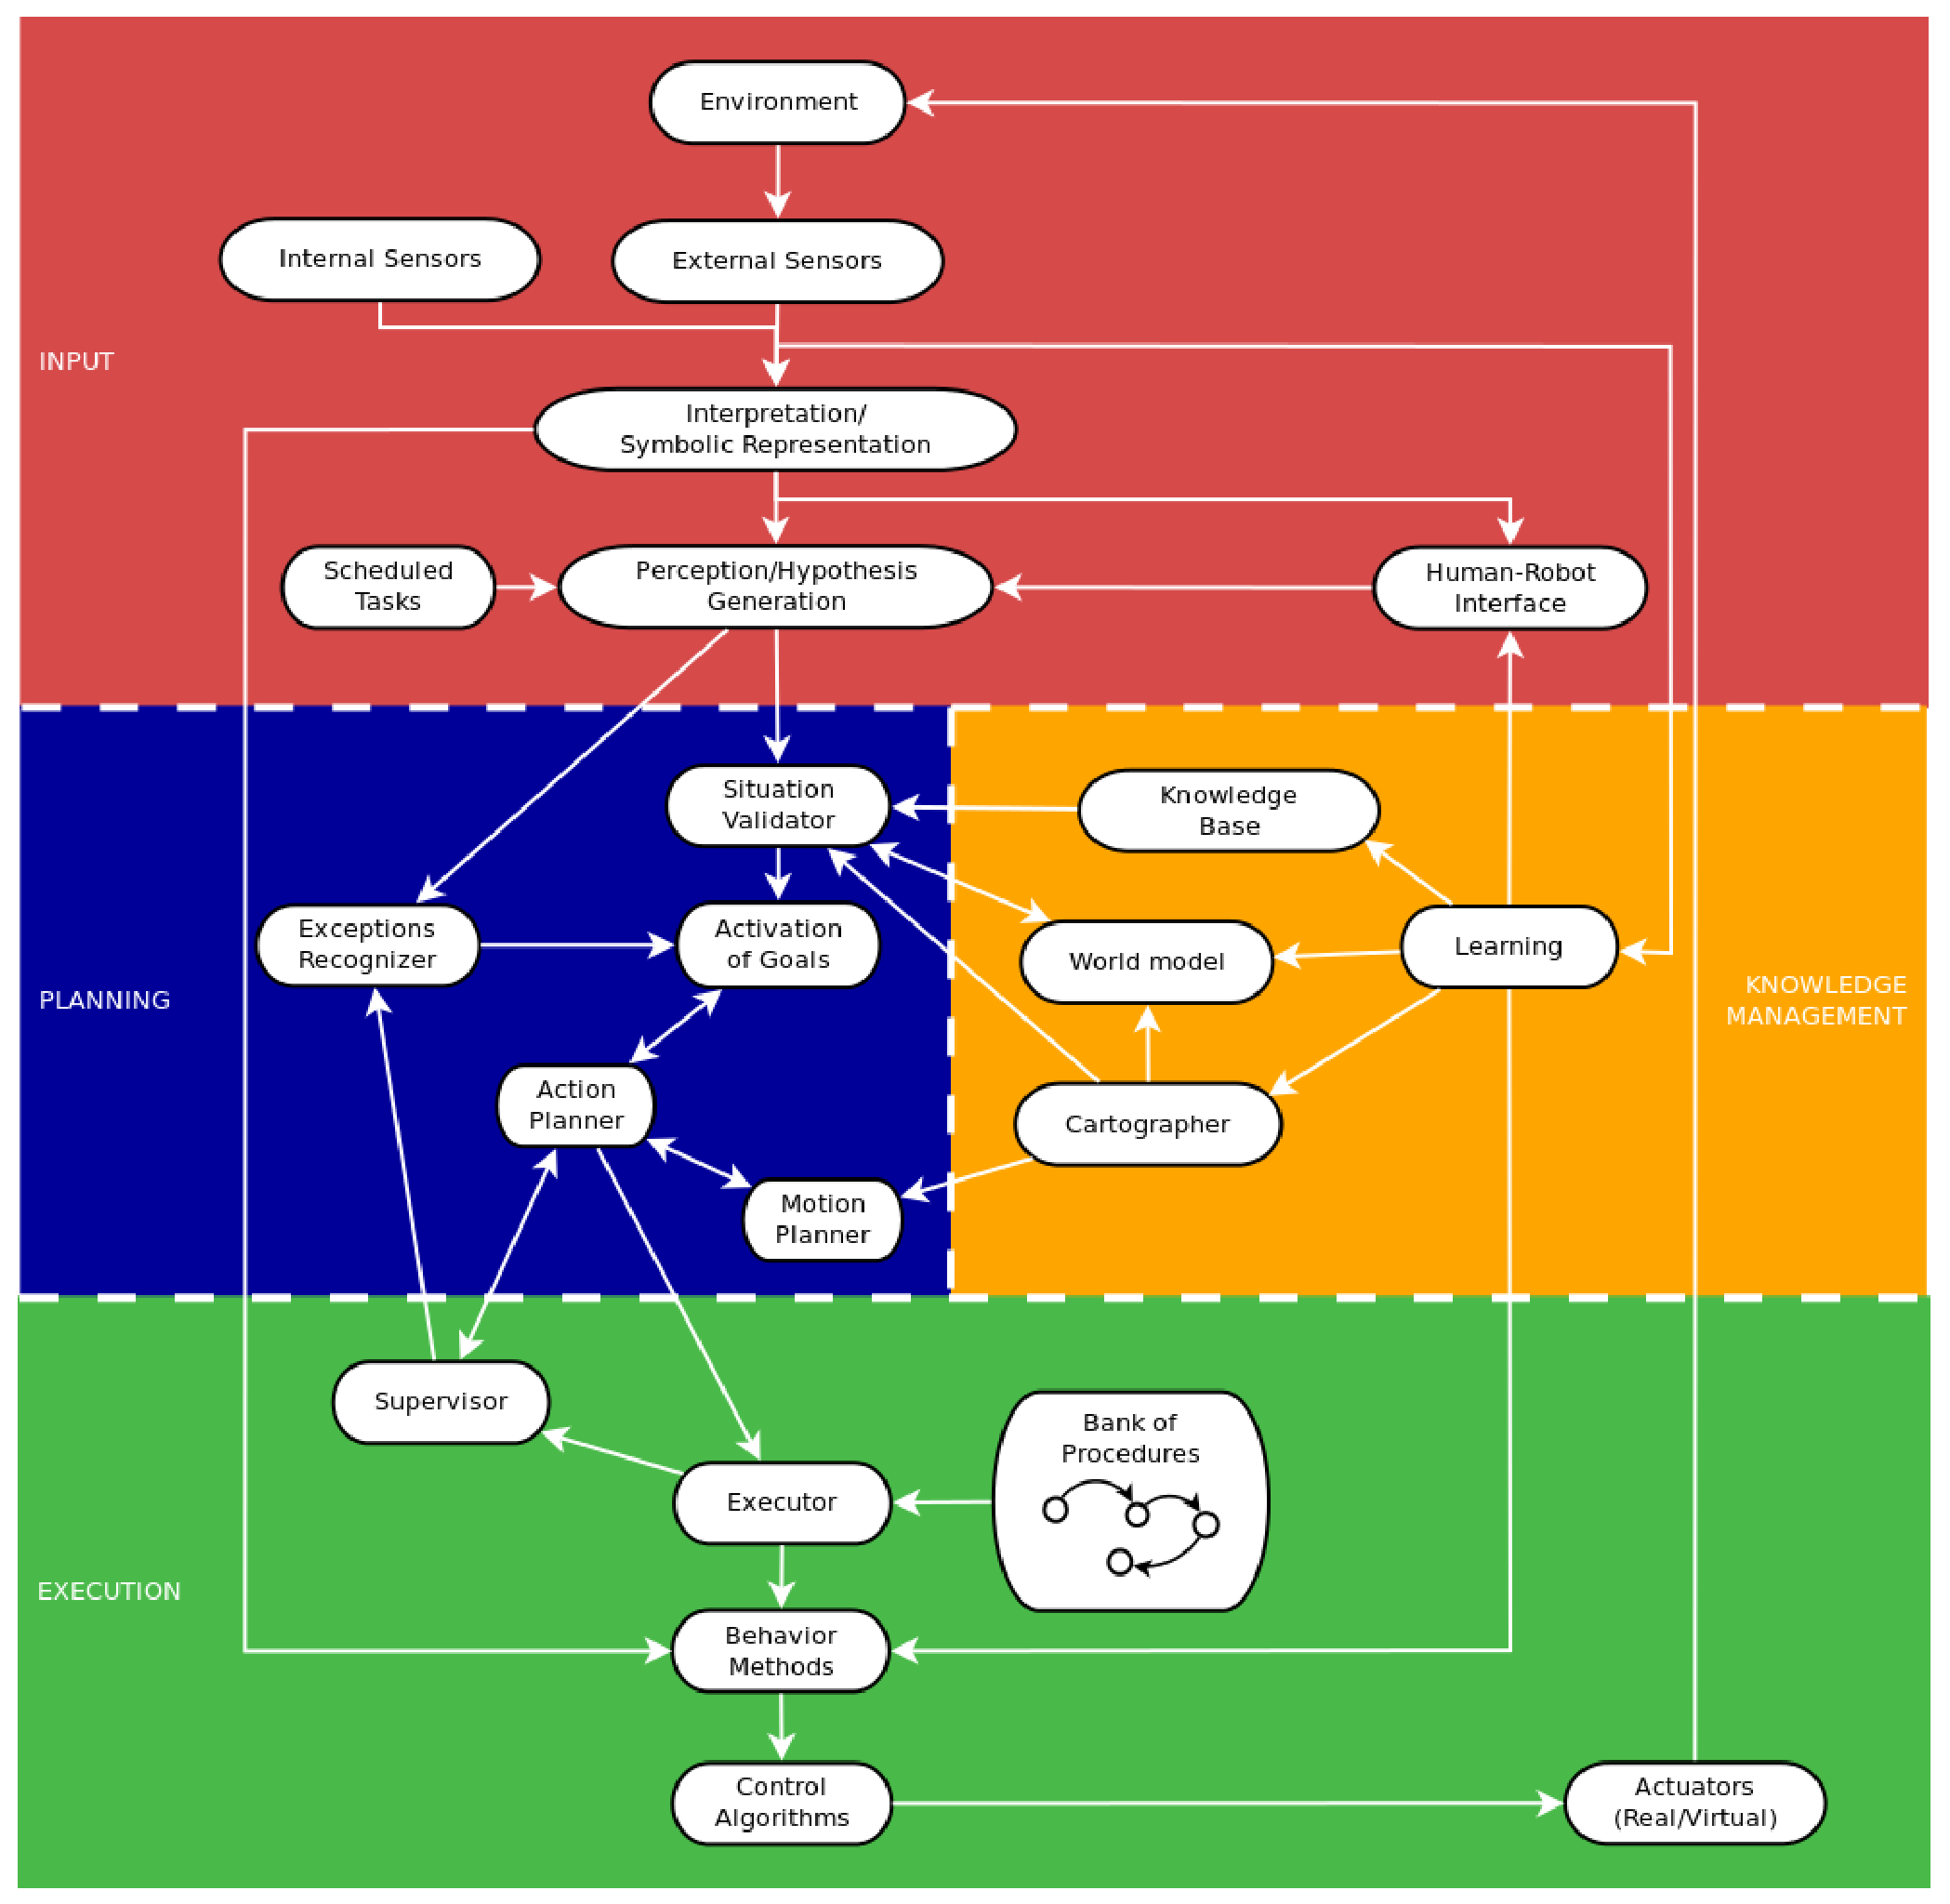
\includegraphics[angle=0, height=10cm, width=10cm]{Figures/ViRBot.eps}
	\caption{Block diagram of the ViRBot architecture.}
	\label{fig:virbot}
\end{figure}


\subsection{Inputs Layer}

This layer process the data from the robot's internal and external sensors, they provide information of the internal state of the robot, along with the external world where the robot interacts.
In some of Justina's designs it has lasers, sonars, infrared, microphones and stereo and RGB-D cameras.
Digital signal processing techniques are applied to the data provided by the internal and external sensors to obtain a symbolic representation of the data, furthermore, to recognize and to process voice and visual data.
Pattern recognition techniques are used to create models of the objects and the people that interact with the robot.
With the symbolic representation this module generates a series of beliefs, that represent the state of the environment where the robot interacts.


\subsection{Planning Layer}

The beliefs generated by the perception module are validated by this layer, it uses the Knowledge Management layer to validate them, thus a situation recognition is created.
Given a situation recognized, a set of goals are activated in order to solve it.
Action planning finds a sequence of physical operations to achieve the activated goals.


\subsection{Knowledge Management Layer}

This layer has different types of maps for the representation of the environment, they are created using 
SLAM techniques.
Also in this layer there is a localization system, that uses the Kalman filter, to estimate the robot's position and orientation.
A rule based system, CLIPS, developed by NASA, is used to represent the robot's knowledge, in which each rule contains the encoded knowledge of an expert.


\subsection{Execution Layer}
This layer executes the actions and movements plans and it checks that they are executed accordingly.
A set of hardwired procedures, represented by state machines, are used to partially solve specific problems, person recognition, object manipulation, etc. The action planner uses these bank of procedures and it joins some of them to generate a plan.


%%%%%%%%%%%%%%%%%%%
%%% CURRENT RESEARCH  %%%
%%%%%%%%%%%%%%%%%%%

\section{Current research}\label{sec:CurrentResearch}
In this section is presented the current research developed in our laboratory to improve the performance of our service robots.

\subsection{Natural language understanding}\label{subsec:NaturalLU}
Natural language understanding is used in order to the service robot interprets the language and then perform an especific task.
One of the main problems using natural language understanding is the representation of meaning.  
We have a framework for defining the semantics. The robot's semantics are therefore instructions that allow it to carry out relevant operations.

Conceptual Dependency (CD) is a theory, developed by Schank \cite{Schank}, for representing the meaning contained in sentences. 
This technique finds the structure and the meaning of a sentence in just one step. 
It is useful to represent sentences using this technique when there is not a strict grammar associated with the sentences, and also when the objective is to make inferences from them.
The CD representation of a sentence is built using conceptual primitives, these represent thoughts and the relationships between thoughts. Using conceptual dependency facilitates the use of inference rules, because many inferences are already contained in the representation itself.
There are several primitives to represent actions, for example two of the more commonly used are the following:

\vspace{.01 in}
		ATRANS: Transfer of an abstract relationship (e.g., give.)

\vspace{.01 in}
		PTRANS: Transfer of the physical location of an object (e.g., go.)
\vspace{.01 in}

Each primitive represents several verbs which have similar meaning. For instance give, buy, steal, and take have the same meaning, i.e., the transference of one object from one entity to another one.
Each primitive is represented by a set of rules and data structures. Basically each primitive contains the following components:
\vspace{.01 in}

	An Actor: He is the one that perform the ACT.
\vspace{.01 in}

	An ACT: Performed by the actor, done to an object.
\vspace{.01 in}

	An Object: The action is performed on it.
\vspace{.01 in}

	A Direction: The location that an ACT is directed towards.
\vspace{.01 in}

	A State: The state that an object is in, and is represented using a knowledge base representation as
facts in an expert system. 
\vspace{.01 in}

	For instance the phrase: {\bf "Robot, please give this book to Mary"}, 
when the verb give is found in the sentence an ATRANS structure is issued.
\vspace{.01 in}

	(ATRANS (ACTOR NIL) (OBJECT NIL) (FROM NIL) (TO NIL))
\vspace{.01 in}

The empty slots (NIL) need to be filled finding the missing elements in the sentence. The actor is the robot, the 
object is the book, etc, and it is represented by the following CD:
\vspace{.01 in}

	(ATRANS (ACTOR Robot) (OBJECT book) (FROM book's owner) (TO Mary))
\vspace{.01 in}


CDs can be use for representing simple actions. It is also well suited for representing commands or simple questions, but it is not very useful for representing complex sentences.
The CD technique were implemented in an expert system.


Much of the human problem solving or cognition can be expressed by IF THEN type production rules. Each rule corresponds to a modular collection of knowledge call chunk. The chunks are organized in loose arrangement with links to related chunk of knowledge, reasoning could be done using rules. 
Each rule is formed by a left side that needs to be satisfied (Facts) and by a right side that produce the appropriate response (Actions).  
\vspace{.01 in}

		IF  Facts  THEN  Actions.
\vspace{.01 in}

When an action is issued by a rule it may become a fact for other rules, creating links to other rules. A system may use thousands of rules to solve a problem, thus it is necessary a special mechanism that will select which rules will be fired according to the presented facts. That mechanism is an Expert System "Engine".
The Inference Engine makes inferences by deciding which rules are satisfied by facts, prioritize the 
satisfied rules, and executes the rule with the highest priority.
This expert system provides a cohesive tool for handling a wide variety of knowledge with support for three different programming paradigms: rule-based, object-oriented, and procedural.
%In the VIRBOT system an expert system maintains a knowledge data base that represents the state of the world.
The data of the humans interacting with the robot, of the objects and the locations is represented using facts that contain several slots with information related with them.
The Robot is able to perform operations like grasping an object, moving itself from on place to another, finding humans, etc. Then the objective of action planning is to find a sequence of physical operations to achieve the desired goal.
These operations are represented by a state-space graph.

In the previous example, when the user says {\bf "Robot, please give this book to Mary"}: 
\begin{itemize}
\item []
	(ATRANS (ACTOR Robot) (OBJECT book) (FROM book's owner) (TO Mary))
\end{itemize}

All the information required for the actions planner to perform its operation is contained in the CD and knowledge data base. 
Our system has been successfully tested in robotics competitions \cite{Savage}, as the RoboCup and RockIn 
\cite{Robocup_2017}, in the category @Home.
In RoboCup@Home 2017 our robot was awarded as the best in Speech and Natural Language Understanding.



\subsection{Facial detection through multiple images using RGB cameras}\label{subsec:FacialReco}
The facial detection is one of the most primordial tasks that a service robot must be able to perform, proof of them is that in the RoboCup@Home there is a test in which the robot must correctly state the number of people who make up a crowd, these people can  be stand, sit and even lie down, the crowd can be composed of very tall people or children and the crowd size can range from 5 to 10 people, so that correctly stating the crowd turns out to be a difficult task to be solved with a single image, that is why we decided to figure out the problem by generating a registered image composed by several images at different angles, in figure \ref {frames} are shown some samples to perform the image registration. Stitching is the process of merging multiple images with fields of view that overlap to produce a registered image. %Most image stitching techniques require almost exact overlaps between images to produce splendid results. 
The image stitching method can be divided into three main phases: image registration, calibration and mixing.

%\begin{itemize}
%	\item \textbf{Registration:}% Involves pairing features in set of images or directly uses alignment methods to search for image alignments that minimize the sum of absolute differences between pixel overlays.
%	\item \textbf{Calibration:} %Image calibration aims to minimize the differences between an ideal lens model and the combination of camera and lens that was used, optical defects such as distortions, different exposures between images, camera response and chromatic aberrations.
%	\item \textbf{Mixing:} %Involves making improvements, including color adjustments. Colors are adjusted between images to set off for differences in exposure. The images are mixed together and the arrangement of the stitching line is done to minimize the visibility of the joints between the images.
%\end{itemize}
\begin {figure}[h]
	\centering
	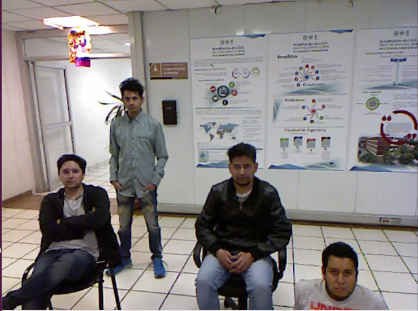
\includegraphics[angle=0, height= 3cm, width=4cm]{Figures/pano3.png}
	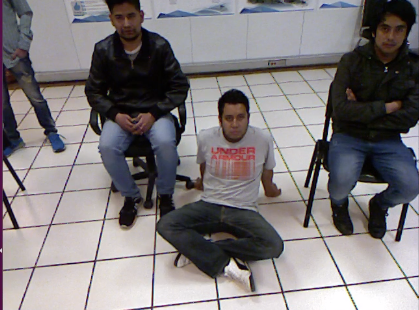
\includegraphics[angle=0, height= 3cm, width=4cm]{Figures/pano2.png}
	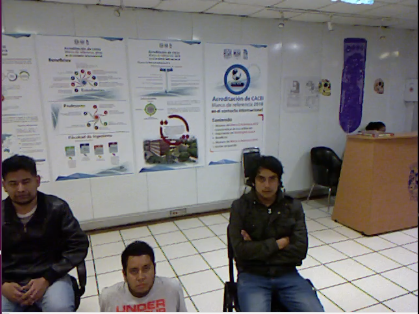
\includegraphics[angle=0, height= 3cm, width=4cm]{Figures/pano1.png}
	\caption{Frames Captured by the Robot at Different Angles.}
	\label{frames}
\end {figure}

The first thing we do in our implementation is to convert the color images to grayscale images, then we use SURF \cite{surf} as a feature detector. The next step is to perform pairing of the detectors using FLANN \cite{flann}, we also execute a computation to obtain the maximum and minimum distances of the points of interest. We later found the homography matrix using RANSAC \cite{ransac}. Finally we combined the images using the homography matrix. All this process is done iteratively, first we start with two images, to the union of those two images we can join another and so on. Once we have the registered image, we work with it to compute the facial detection. The results are shown in figure \ref{pano_image}.





\begin{figure}[h]
	\centering
	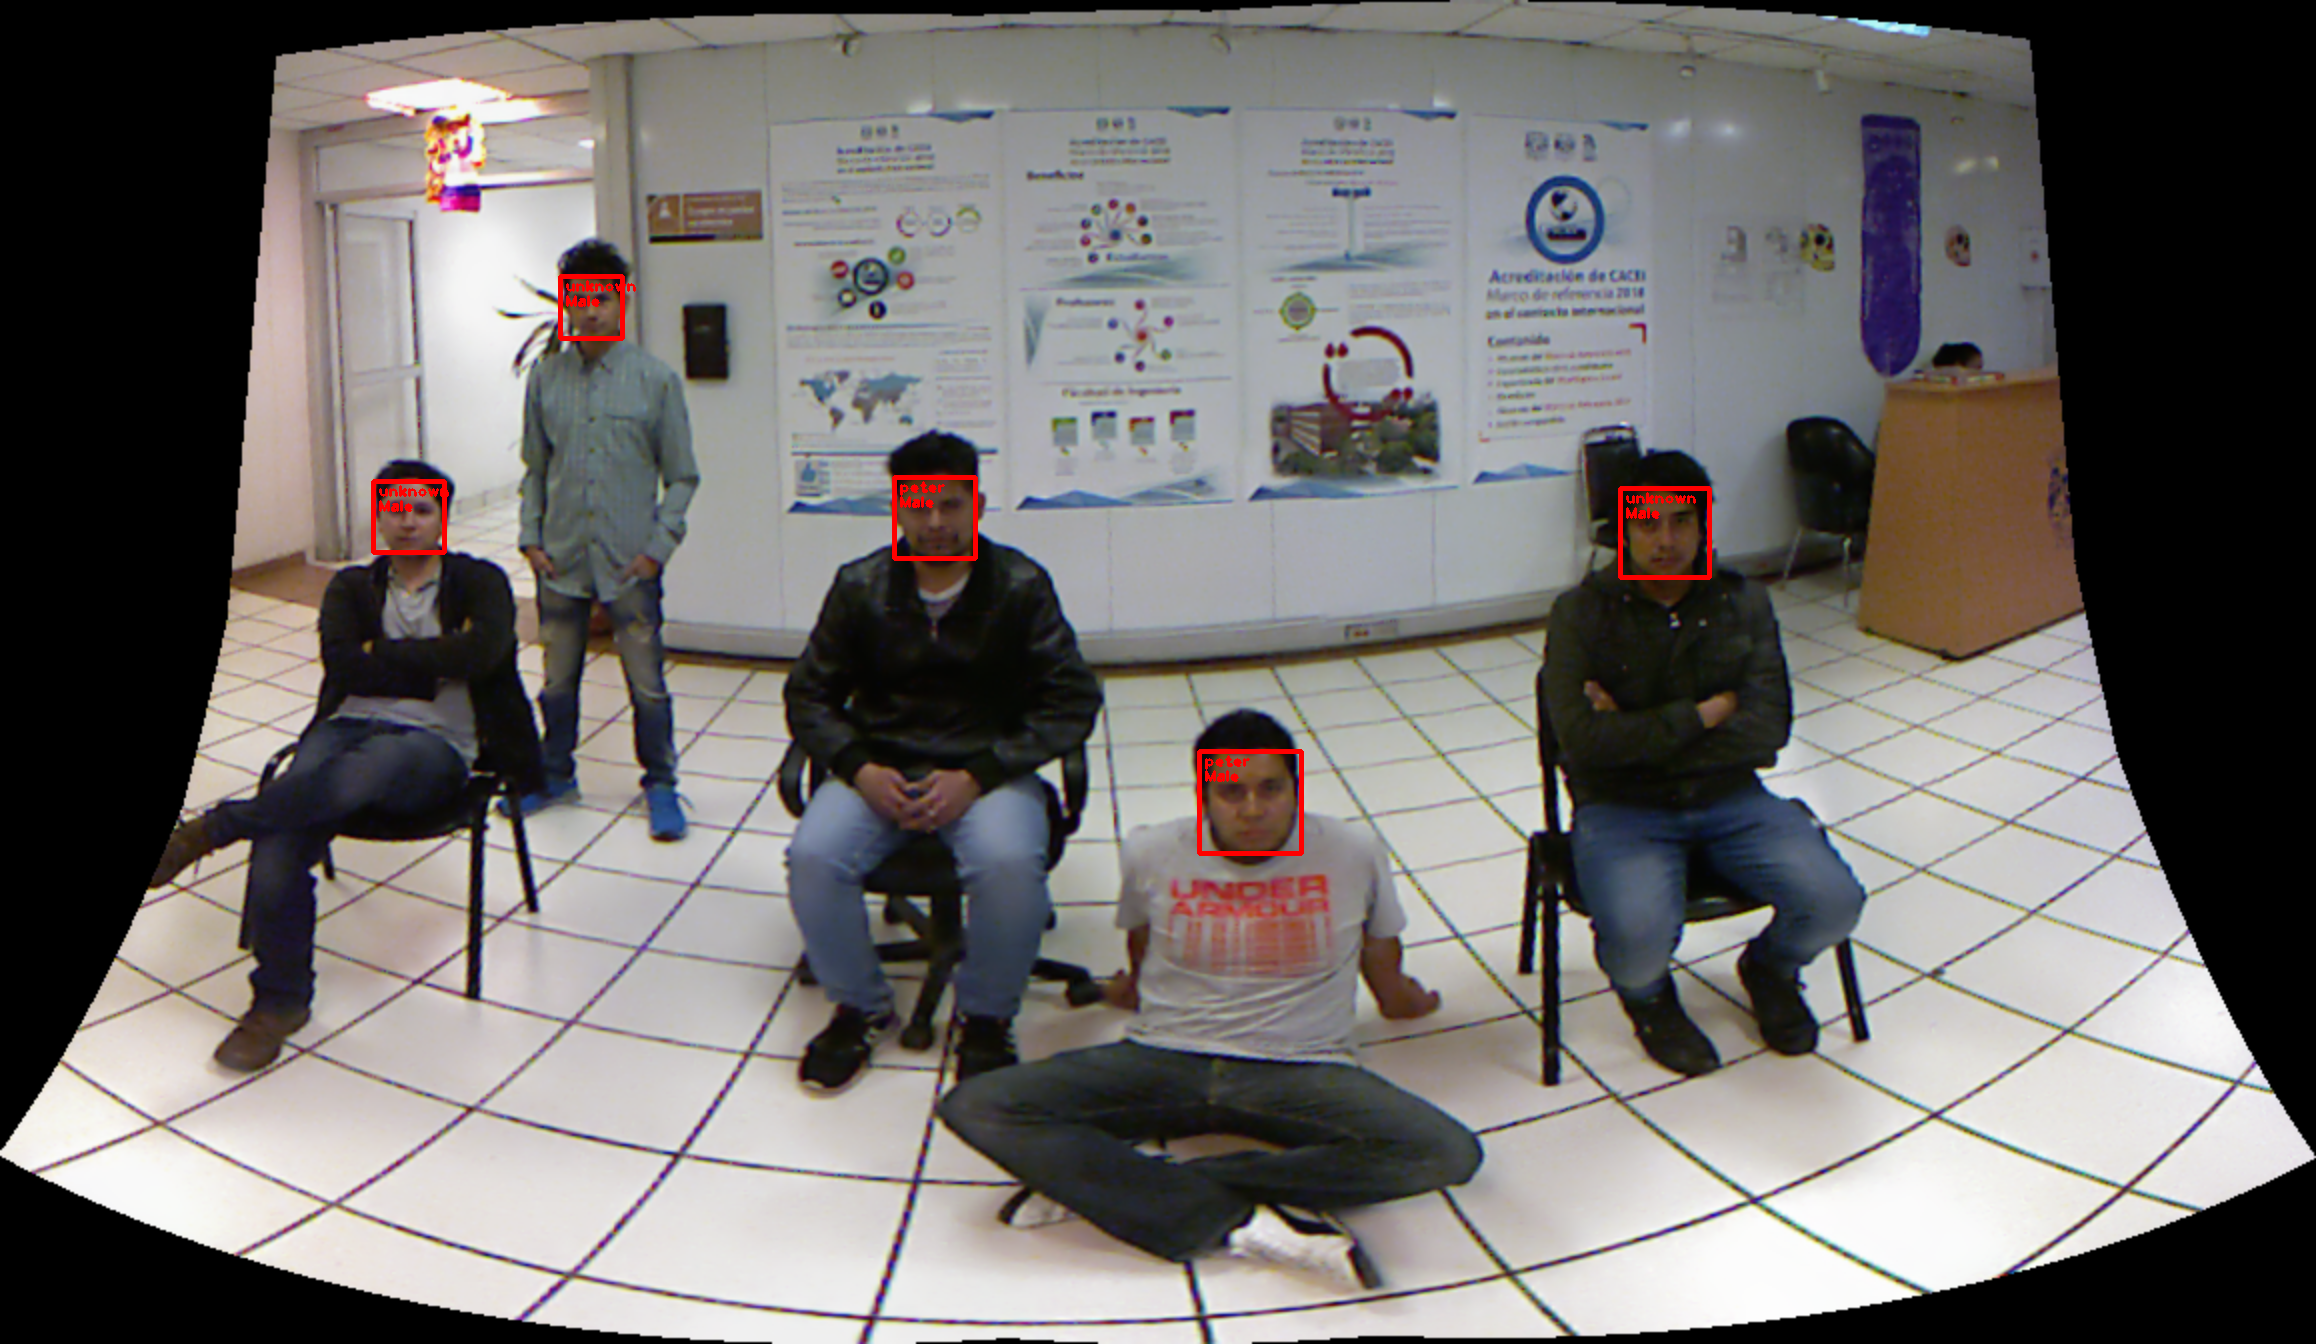
\includegraphics[angle=0, height=3.7cm, width=8cm]{Figures/sceneComplete_pano.png}
	\caption{Facial Detection on a Registered Image.}
	\label{pano_image}
\end{figure}


 


\subsection{Sound Source Localization}\label{subsec:SoundSource}

\begin{wrapfigure}{r}{0.4\textwidth}
	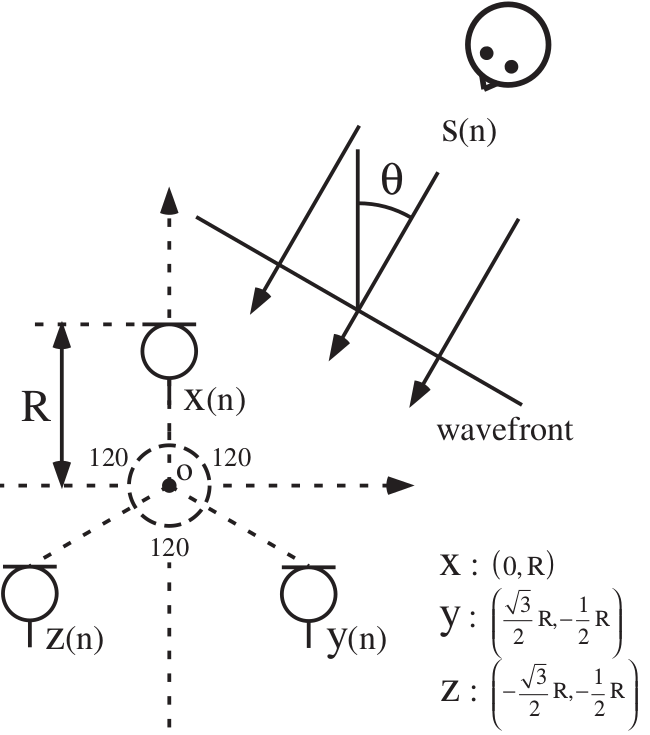
\includegraphics[angle=0, height= 4cm, width= 4.5cm]{Figures/array.png}
	\caption{Equilateral triangular arrangement \cite{hioka2003}.}
	\label{F_array}
\end{wrapfigure}
The Sound Source Localization (SSL) is performed by estimating the direction of arrival (DOA) of the voice signals of people who are in unknown positions around the robot. Considering the DOA estimate is required over an angular range of $[0,2\pi)$, a triangular arrangement of microphones was used, as shown in figure \ref{F_array}.



For the DOA estimation it is crucial to obtain the phase information present in the signals of each of the microphones \cite{karbasi2006}. In order to obtain accurate information about the signal offset in each of the microphones, an MCU was used for the acquisition and processing of the signals, the MCU used is the TMS320F28377S, which has two 12-bit analog-to-digital (ADC) converters, each of these ADCs has seven channels with independent conversion starts (SOC), with these ADCs can be obtained up to 1.1 MSPS \cite{DTASHT2}. The DOA calculation is performed using the cross-power spectral density (CPSD) between pairs of microphones, the CPSD between signals  $x_1$ and $x_2$ is obtained as:
\begin{equation}
	G_{12}(\omega) = X_1^{*}(\omega) X_2(\omega) = P(\omega)e^{-j\omega \tau}
\end{equation} 

being $X_1(\omega)$ and $X_2(\omega)$ the Fourier transforms (FT) of $x_1(n)$ y $x_2(n)$, respectively.%i.e., if you have two signals $x_1(n)$ and $x_2(n)$ defined as:
%\begin{equation}
%	x_1(n) = s(n)+\eta_1(n)
%\end{equation}
%
%\begin{equation}
%	x_2(n) = s(n-\tau)+\eta_2(n)
%\end{equation}

%where $s(n)$ is the signal of interest, $\eta_1(n)$ and $\eta_2(n)$ are uncorrelated noise signals, the CPSD between signals $x_1$ and $x_2$ is obtained as:
In the case of the triangular arrangement, there will be three pairs of microphones, so there are three CPSDs. Using the three previous CPSDs, the integrated cross-spectrum can be obtained as:
\begin{equation} \label{eq_doa}
	G_{\phi,\theta}^{(\omega)} (\theta,\phi) = G_{x2y}^{(\omega)}(\phi)G_{xy}^{(\omega)}(\theta)+G_{yz}^{(\omega)}(\theta)+G_{z2y}^{(\omega)}(\phi)G_{zx}^{(\omega)}(\theta)
\end{equation}


The above equation has its maximum when $\phi=\theta$, In this way, the angle of arrival is located at the angle $\phi$ that maximizes the equation (\ref{eq_doa}).

%%%%%%%%%%%%%%%%%%%%%%%%%%
%%%  CONCLUSION AND FUTURE WORK  %%%
%%%%%%%%%%%%%%%%%%%%%%%%%%

\section{Conclusions and future work}\label{sec:conclusions}
It is clear, that during the 10 years in which our team Pumas has been participated in the RoboCup and 2 years in the Rockin \cite{Robocup_2017} in the category @Home, the performance and research developed, in the service robot area, in our laboratory has been improved considerably.
Our service robot architecture, the VIRBOT, has been evolving according to the requirement that these robotics competitions asked each year.
In these years, the full system has been improved, both in hardware and software, having reliable performance and showing promising results. Particularly, this year, we have a new omnidirectional mobile base for navigation and a new torso. 
In terms of software, we have change the way of conceiving the tests of the competition: from static state machines to inferred action planning generated by a rule based system. 
As for future work, the task of following humans will be improved by combining vision algorithms using the Kinect sensor and our current system tha use a laser. Also, it will be explored topics as the memory and enviromental reasoning of the robot, in order to explain things that hapenned in the past. Moreover we are working in a mask with lights that serves as an interface to express different emotions.
\bibliographystyle{unsrt}
\bibliography{bibliography,justina}

\begin{thebibliography}{1}


\bibitem{virbot}
{\em ViRbot: A System for the Operation of Mobile Robots}, Savage, Jesus and et al, RoboCup 2007: Robot Soccer World Cup XI,
pp 512-519, Springer Berlin Heidelberg, 2007.

\bibitem{muller}
{\em The Design of Intelligent Agents: A Layered Approach}, Muller, Jorg P,Springer-Verlag New York, Inc.1997.

\bibitem{Schank}
{\em Conceptual dependency and its descendants}, Steven L. Lytinen, Computers \& Mathematics with Applications, 1992.

\bibitem{Savage}
{\em The Role of Robotics Competitions for the Development of Service Robots}, 
 Jesus Savage, Marco Negrete, Mauricio Matamoros, Jesus Cruz,
IJCAI'16, Workshop on Autonomous Mobile Service Robots, New York, USA, 2016.

\bibitem{Robocup_2017}
{\em RoboCup@Home} http://www.robocupathome.org
\\
{\em Rockin} http://rockinrobotchallenge.eu/home.php

\bibitem{surf}
{\em SURF: Speeded Up Robust Features}, Herbert B., Andreas E., Tinne T., Luc Van G., Computer Vision and Image Understanding (CVIU), 110(3): 346-359, 2008.

\bibitem{flann}
{\em Fast Approximate Nearest Neighbors with Automatic Algorithm Configuration}, Marius Muja and David G. Lowe, International Conference on Computer Vision Theory and Applications (VISAPP'09), 2009.

\bibitem{ransac}
{\em  Random Sample Consensus: A Paradigm for Model Fitting with Applications to Image Analysis and Automated Cartography}, Fischler, Martin A. and Bolles, Robert C., Commun. ACM, 24(6): 381-395, 1981.

\bibitem{hioka2003}\textit{DOA estimation of speech signal using equilateral-triangular microphone array}, Yusuke Hioka and Nozomu Hamada, 8th European Conference on Speech Communication and Technology (EUROSPEECH 2003), 2003.

\bibitem{karbasi2006}\textit{A DOA estimation method for an arbitrary triangular microphone arrangement}, Amin Karbasi and Akihiki Sugiyama, 14th European Signal processing Conference (EUSIPCO 2006), 2006.

\bibitem{DTASHT2} 
{\em TMS320F2837xS Data Sheet} http://www.ti.com/lit/ds/sprs881b/sprs881b.pdf


\end{thebibliography}

\section{Team Information}\label{sec:TeamInfo}
{\bf Name of Team:} 


Pumas\\
{\bf Contact Information:}


Jesus Savage


Bio-Robotics Laboratory


School of Engineering 


National Autonomous University of Mexico


robotssavage@gmail.com\\
{\bf Web Site:}


http://biorobotics.fi-p.unam.mx\\
{\bf Team Members:}


Jesus Savage, Reynaldo Martell, Hugo Estrada, Marco Negrete, Julio Cruz,


Jesus Cruz, Jose Cruz, Edgar Vazquez, Jaime Marquez, Edgar Silva, Manuel


Pano, Luis Alvarez, Mauricio Matamoros\\
{\bf Description of Hardware:}

Justina's Robotics Architecture (cf. section 2)\\
{\bf Description of Software:}

Most of our software and configurations are open-source and can found at: 

https://github.com/RobotJustina/JUSTINA\\

\begin{tabular}{l@{\extracolsep{3 cm}}  r}
 \hline                 
   Operating System & Ubuntu 16.04 LTS; Windows 7 VM \\
   Middleware & ROS Kinetic; Blackboard\\
   SLAM & ROS Gmapping\\
   Navigation & Navigation using Kinect + Ocupancy grid + A*\\
   Object Recognition & Histogram Disparity\\
   Face Detection & Haar Cascades\\
   People Detection & OpenPoses\\
   Face Recognition & EigenFaces\\
   Speech Synthesis & Loquendo\\
   Speech Recognition & Microsoft Speech Recognition\\
   Inference Engine & CLIPS\\
 \hline  
 \end{tabular}
	


\end{document} 
